%
% $Id: $
%
%
% Compilar a .pdf con LaTeX (pdflatex)
% Es necesario instalar Beamer (paquete latex-beamer en Debian)
%

%
% Gráficos:
% Los gráficos pueden suministrarse en PNG, JPG, TIF, PDF, MPS
% Los EPS deben convertirse a PDF (usar epstopdf)
%

\documentclass{beamer}
\usetheme{Warsaw}
\usebackgroundtemplate{
\includegraphics[width=\paperwidth]{format/libresoft-bg-soft.png}}
\usepackage[spanish]{babel}
\usepackage[utf8]{inputenc}
\usepackage{graphics}
\usepackage{amssymb} % Simbolos matematicos

%\definecolor{libresoftgreen}{RGB}{162,190,43}
%\definecolor{libresoftblue}{RGB}{0,98,143}

%\setbeamercolor{titlelike}{bg=libresoftgreen}

%% Metadatos del PDF.
\hypersetup{
  pdftitle={Economic Aspects of Libre Software / Master on Libre Software (URJC)},
  pdfauthor={Jesus M. Gonzalez-Barahona, Felipe Ortega},
  pdfcreator={GSyC/LibreSoft, Universidad Rey Juan Carlos},
  pdfproducer=PDFLaTeX,
  pdfsubject={},
}
%%

%\includeonly{presentation}
%\includeonly{introduction}
%\includeonly{innovation}

%\includeonly{oss-business-models-statements,questions-video-benkler}
\includeonly{questions-video-leadbeater}

\AtBeginSection[]
{
\begin{frame}<beamer>
\begin{center}
{\Huge \insertsection}
\end{center}
\end{frame}
}

\begin{document}

\title{Economic Aspects of Libre Software }
\subtitle{Master on Libre Software (URJC) \\
\url{http://master.libresoft.es}}
\author{Jesus M. Gonzalez-Barahona, Felipe Ortega}
\institute{jgb@gsyc.es jfelipe@libresoft.es\\
@jgbarah @felipe
GSyC/LibreSoft, Universidad Rey Juan Carlos}

\date{November 2010}

\frame{
\maketitle
\begin{center}

\includegraphics[width=6cm]{format/gsyc-urjc}
\end{center}
}


% Si el titulo o el autor se quieren acortar para los pies de página
% se pueden redefinir aquí:
%\title{Titulo corto}
%\author{Autores abreviado}


%% LICENCIA DE REDISTRIBUCION DE LAS TRANSPAS
\frame{
~
\vspace{3cm}

\begin{flushright}
\copyright 2010 Jesus M. Gonzalez-Barahona, Felipe Ortega. \\

Some rights reserved. \\
This document is distributed under the \\
Creative Commons Attribution-ShareAlike 3.0 licence, \\
available in \\
\url{http://creativecommons.org/licenses/by-sa/3.0}

The original version of this document is available at \\
\url{http://master.libresoft.es}
\end{flushright}
}
%%

%% presentation.tex
%%
%% Presentation of the course ``Master Thesis" of the Official Master on Libre Software (URJC)
%% http://master.libresoft.es
%%

%%---------------------------------------------------------------------
%%---------------------------------------------------------------------

\section{Presentation of the Master Thesis Course}

%%---------------------------------------------------------------

\begin{frame}
\frametitle{Administrative data}

\begin{itemize}
\item Both semesters, 12 ECTS credits
\item Teachers:
  \begin{itemize}
  \item Gregorio Robles (grex at gsyc.urjc.es)
  \item Jesus M. Gonzalez-Barahona (jgb at gsyc.urjc.es)
  \item Departamento de Sistemas Telem�ticos y Computaci�n (GSyC)
  \item Rooms 109 and 120 Departamental II (M�stoles campus)
  \item Room 103 Biblioteca (Fuenlabrada campus)
  \end{itemize}
\item Schedule: see Calendar
\item Sessions:
  \begin{itemize}
  \item Classroom 215, Aulario II, Fuenlabrada campus
  \end{itemize}
\item Moodle course (please, join it as soon as possible): \\
  \url{http://docencia.etsit.urjc.es/moodle/course/view.php?id=134}
\end{itemize}
\end{frame}

%%---------------------------------------------------------------

\begin{frame}
\frametitle{Goals}

Primary Goal: 
To apply the lessons and practices learned in this master
to a real problem

Secondary goal
To do it in one term

\end{frame}

%%---------------------------------------------------------------


\begin{frame}
\frametitle{Evaluation}

\begin{itemize}
\item 
\end{itemize}

\end{frame}

%%---------------------------------------------------------------

\begin{frame}
\frametitle{}

\begin{itemize}
\item 
\end{itemize}

\end{frame}

%%---------------------------------------------------------------

\begin{frame}
\frametitle{}

\begin{itemize}
\item 
\end{itemize}

\end{frame}

%%---------------------------------------------------------------

\begin{frame}
\frametitle{}

\begin{itemize}
\item 
\end{itemize}

\end{frame}


%%---------------------------------------------------------------

\begin{frame}
\frametitle{Some references}

\begin{itemize}
\item  \\
  \url{}
\item Introduction to libre software (book) \\
  \url{http://curso-sobre.berlios.de/introsobre}
\end{itemize}

\end{frame}

%% introduction.tex
%%
%% Introduction to the course ``Economic aspects'' of the
%%   Official Master on Libre Software (URJC)
%%   http://master.libresoft.es

%%---------------------------------------------------------------------
%%---------------------------------------------------------------------
\section{Introduction and motivation}

%%---------------------------------------------------------------

\begin{frame}
\frametitle{The growth of libre software (1)}

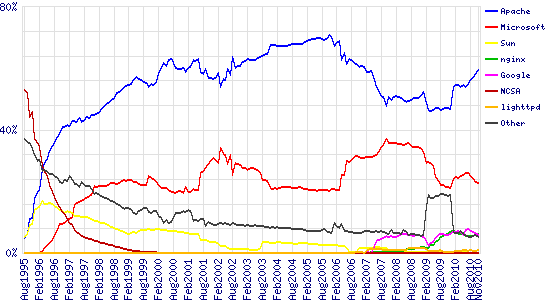
\includegraphics[height=6cm]{webservers-share-2010-11}

\begin{flushright}
Netcraft Survey, November 2010 \\
{\small \url{http://news.netcraft.com/archives/2010/11/05/november-2010-web-server-survey.html}}
\end{flushright}
\end{frame}

%%---------------------------------------------------------------

\begin{frame}
\frametitle{The growth of libre software (2)}

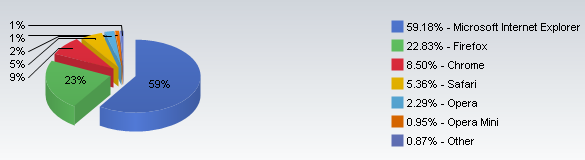
\includegraphics[height=3.5cm]{webbrowsers-share-2010-10}

\begin{flushright}
Net Market Share Report, October 2010 \\
{\small \url{http://www.netmarketshare.com/}}
\end{flushright}
\end{frame}

%%---------------------------------------------------------------

\begin{frame}
\frametitle{The growth of libre software (3)}

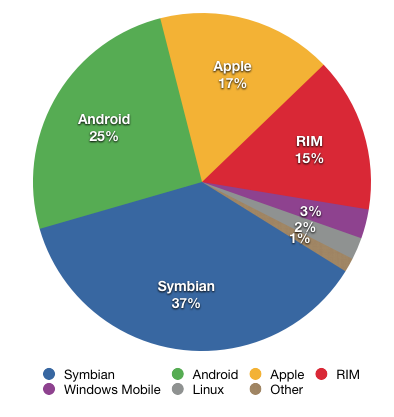
\includegraphics[height=5cm]{smartphone-share-gartner-2010-q3}

\begin{flushright}
Competitive Landscape: Mobile Devices, 3Q10 (Gartner)\\
Worldwide smartphone sales, 3rd Q 2010 \\
{\small \url{http://www.gartner.com/it/page.jsp?id=1466313}} \\
(graph from Wikimedia Commons)
\end{flushright}
\end{frame}


%%---------------------------------------------------------------

\begin{frame}
\frametitle{The adoption of libre software (1)}

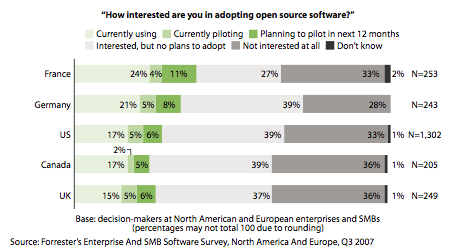
\includegraphics[height=5cm]{adoption-interest-forrester-2007-q3}

\begin{flushright}
Open Source Adoption: Notes From The Field \\
(Forrester, July 2008) \\
{\small \url{http://www.forrester.com/rb/Research/open_source_adoption_notes_from_field/q/id/46279/t/2}} 
\end{flushright}
\end{frame}

%%---------------------------------------------------------------

\begin{frame}
\frametitle{The adoption of libre software (2)}

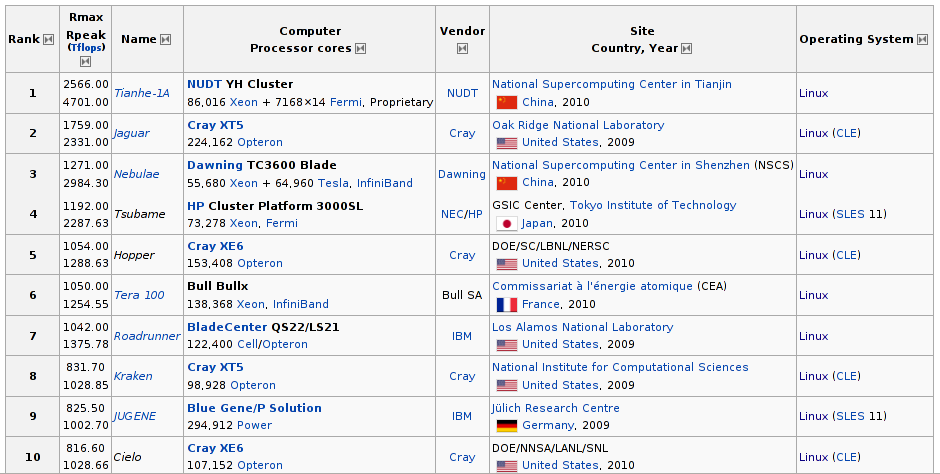
\includegraphics[height=6cm]{top-10-supercomputers-2010-11}

\begin{flushright}
36th TOP500 List (November 2010) \\
{\small \url{http://www.top500.org} \url{http://en.wikipedia.org/wiki/TOP500}} 
\end{flushright}
\end{frame}

%%---------------------------------------------------------------

\begin{frame}
\frametitle{The adoption of libre software (3)}

\begin{center}
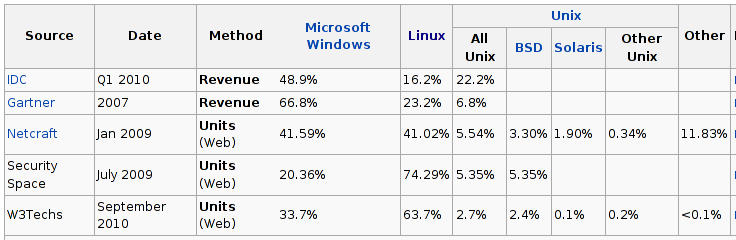
\includegraphics[height=4cm]{server-os-share-2010}
\end{center}

\begin{flushright}
Server market share, operating systems (Wikipedia) \\
{\footnotesize \url{http://en.wikipedia.org/wiki/Usage_share_of_operating_systems}} 
\end{flushright}
\end{frame}

%%---------------------------------------------------------------

\begin{frame}
\frametitle{The adoption of libre software (4)}

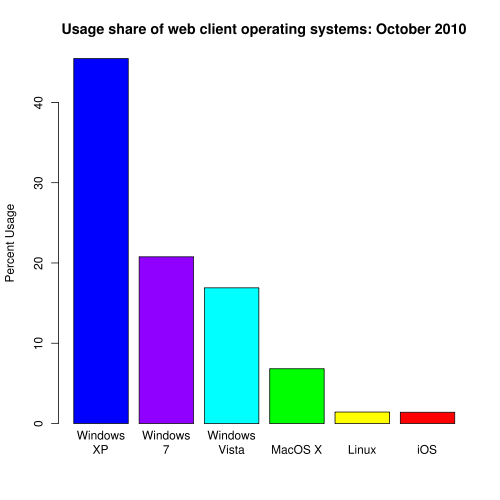
\includegraphics[height=6cm]{desktop-os-marketshare-2010-10}

\begin{flushright}
Usage share of web client operating systems \\
(Wikipedia, October 2010, median of usage studies) \\
{\small \url{http://en.wikipedia.org/wiki/Usage_share_of_desktop_operating_systems}} 
\end{flushright}
\end{frame}

\end{frame}



\section{Supporting innovation with free software}

%%---------------------------------------------------------------

\begin{frame}
\frametitle{Summary}

\begin{quote}
Free software has shown, in several areas, how it may be a powerful tool for supporting innovation processes, and the dissemination of its results. This presentation will show the relationship between free software and innovation, and some of the characteristics of innovation processes supported by free software.
\end{quote}

\end{frame}



%%---------------------------------------------------------------

\begin{frame}
\frametitle{What is innovation?}

\begin{itemize}
\item Technological advance subdivided into two phases:

  \begin{itemize}
  \item Invention (scientific breakthrough): research
  \item Innovation (commercialization of the invention): development
  \end{itemize}

  \begin{flushright}
    Schumpeter (1934), attributed by Nelson and Winter (1982)
  \end{flushright}

\item Innovation: process by which research results (which may be new technologies) are applied to existing products or lead to new products.
\end{itemize}

\end{frame}

%%---------------------------------------------------------------

\begin{frame}
\frametitle{Free software and open innovation}

\begin{quote}
``Open innovation is a paradigm that assumes that firms can and should use external ideas as well as internal ideas, and internal and external paths to market, as the firms look to advance their technology''
\end{quote}

\begin{flushright}
''Open Innovation: The new imperative for creating and profiting from technology'', Chesbrough, H.W. (2003)
\end{flushright}

Management challenges:

\begin{itemize}
\item Maximization of the use of internal innovation
\item Incorporation of external innovation
\item Motivation of a supply of external innovation. 
\end{itemize}

\end{frame}

%%---------------------------------------------------------------

\begin{frame}
\frametitle{Patterns of open innovation in free software}

Companies use free software in their open innovation strategy \\
(based in [WestGallagher2006]):

\begin{itemize}
\item Pooled research \\
  Pool resources to innovate in a common platform, exploit results
\item Spinouts \\
  Release some non-core innovation in a separate body, but stay involved
\item Selling complements \\
  Income from complements, shared innovation in a common core
\item Donated complements \\
  Income from a core innovation, seek donated labor for
valuable complements
\end{itemize}

\end{frame}

%%---------------------------------------------------------------

\begin{frame}
\frametitle{Case study: Pooled research (Linux, Mozilla)}

\begin{itemize}
\item Firms donate R\&D
\item Firms exploit pooled R\&D of all contributors
\item Mozilla: IBM, HP, Sun, etc.
\item Linux: computers vendors, microprocessor manufacturers, Linux distributors, etc.
\item Maximization: concentrate in their own needs
\item Incorporation: shared technology in their products
\item Motivation: pool of contributors assumed
\end{itemize}

\end{frame}

%%---------------------------------------------------------------

\begin{frame}
\frametitle{Case study: Spinouts (Eclipse, OpenSolaris)}

\begin{itemize}
\item Transformation of internal development in external free software project
\item ``Donation'' of research results, but maintaining involvement
\item Project may generate demand for other products
\item De-facto standards (no need to reimplement to conform with others)
\item Maximization of impact of non-core technologies
\item Incorporation of contributions by third parties
\item Motivation: self-sustainable (or less resource-consuming) communities
\end{itemize}

\begin{flushright}
\url{http://www.eclipse.org}
\end{flushright}
\end{frame}

%%---------------------------------------------------------------

\begin{frame}
\frametitle{Case study: Selling complements (Apache, Konqueror, Android)}

\begin{itemize}
\item Some components comoditized, profit from others (rapidly evolving, difficult to imitate)
\item IBM using Apache httpd for its WebSphere
\item Apple using Konqueror for Safari
\item Google using Linux for expanding to mobile adds and apps
\item (in both cases, contributing back with innovation)
\item Maximization by centering on core products
\item Incorporation of ``free'' external innovation
\item Motivation: self-sustainable (or less resource-consuming) communities
\end{itemize}

Related case: dual licensing, the complement is the proprietary version (e.g., MySQL)

\begin{flushright}
\url{http://httpd.apache.org} \\
\url{http://www.konqueror.org} \\
\url{http://www.android.com}
\end{flushright}

\end{frame}

%%---------------------------------------------------------------

\begin{frame}
\frametitle{Case study: Donated complements (Early BSD Unix, Matlab Central)}

\begin{itemize}
\item Free software components for a proprietary core
\item Heavily based on the interest of a community, but can be promoted
\item Maximization: more value for internal innovation (core product)
\item Incorporation: complements are attracted innovation
\item Motivation: developers involved in the core product, but willing more functionality
\end{itemize}

\begin{flushright}
\url{http://www.mathworks.com/matlabcentral}
\url{http://en.wikipedia.org/wiki/Berkeley_Software_Distribution}
\end{flushright}
\end{frame}

%%---------------------------------------------------------------

\begin{frame}
\frametitle{Free software and community innovation}

Moving to the perspective of the community (as opposed to the firms)

\begin{itemize}
\item Self-sustainable innovation communities
\item Each actor, different motivations
\item Win-win situations when research results flow freely
\item Some rules may help to ``enforce'' free circulation (eg: GPL)
\item Relatively small set of resources may unleash huge potentials
\end{itemize}

\end{frame}

%%---------------------------------------------------------------

\begin{frame}
\frametitle{Case study: GNU/Linux installation process}

\begin{itemize}
\item As opposed to other OSs, GNU/Linux has usually to be installed
\item Continuous improvement of the process
  \begin{itemize}
  \item 1990s: difficult (bad hw support, little flexibility, too specific)
  \item early 2000s: simple (most hw supported, hw-detection libraries, flexible, extensible tools, first live distros)
  \item late 2000s: distro-on-stick, distro-on-file, quick-start, modular systems
  \end{itemize}
\item Collaborative effort by distribution vendors, volunteers, hw vendors, etc.
\item Actors are competing while collaborating
\end{itemize}

\end{frame}

%%---------------------------------------------------------------

\begin{frame}
\frametitle{Case study: KDE, GNOME}

\begin{itemize}
\item Many actors interested in having free software desktops
\item Two main competing systems (GNOME, KDE), with points of contact (FreeDesktop).
\item Volunteers collaborating with companies
\item Companies benefit, and benefit of contributing back (Sun, IBM, Nokia, etc.)
\item Each system composed by an ecosystem of programs, continuously varying
\item Distribution vendors have key interest
\end{itemize}

\end{frame}

%%---------------------------------------------------------------

\begin{frame}
\frametitle{Case study: gvSIG}

\begin{itemize}
\item Created by a public administration (Comunidad de Valencia)
\item Originally, satisfying needs of the creator
\item Other parties joined, contributing small (but valuable) assets
\item A community is created around the core gvSIG system
\item Currently competing head-to-head with other systems in the area
\item Needs of Comunidad de Valencia now provided by a market...
\item ...as is the case of many other parties in the community
\end{itemize}

\begin{flushright}
\url{http://gvsig.org}
\end{flushright}

\end{frame}

%%---------------------------------------------------------------

\begin{frame}
\frametitle{Some final notes}

\begin{itemize}
\item Free software can boost innovation
\item Parties with specific interests have found ways of benefiting
\item Communities of interest can also benefit
\item Strong ties with open innovation concepts
\item New world, new rules: innovation can be an asset that is maximized by sharing it
\end{itemize}

\end{frame}


%%---------------------------------------------------------------

\begin{frame}
\frametitle{References (1)}

\begin{itemize}
\item [WestGallagher2006]
  ``Patterns of Open Innovation in Open Source Software'' \\
  Joel West, Scott Gallagher \\
  (in ``Open Innovation: Researching a New Paradigm'', \\
  Oxford University Press, 2006) \\
  {\small \url{http://openinnovation.haas.berkeley.edu/ranp_chapters/05.pdf}}
\item ``Internet, Innovation, and Open Source: Actors in the Network'' \\
  Ilkka Tuomi \\
  {\small \url{http://citeseerx.ist.psu.edu/viewdoc/download?doi=10.1.1.145.4865&rep=rep1&type=pdf}}
\end{itemize}

\end{frame}


%%---------------------------------------------------------------

\begin{frame}
\frametitle{References (2)}

\begin{itemize}
\item ``Charles Leadbeater on innovation'', TED Talks, \\
  {\small \url{http://www.ted.com/talks/charles_leadbeater_on_innovation.html}}
\item Yochai Benkler on the new open-source economics \\
  {\small \url{http://www.ted.com/talks/yochai_benkler_on_the_new_open_source_economics.html}}
\end{itemize}
\end{frame}



% Assignments and activities
%%

\section{Assignment: Ten myths about FLOSS business models}


\begin{frame}
\frametitle{Dynamics and goals}

\begin{itemize}
\item Statements based on ``Ten myths about FLOSS business models'', by Carlo Daffara \\
\url{http://www.groklaw.net/articlebasic.php?story=20070828132340846}
\item Each one can be right or wrong (or arguable).
\item Work in groups to give simple answers supporting or rebating the statement.
\item Document your answers with factual arguments, if possible (links, data, etc.).
\end{itemize}
\end{frame}

%%%%%%%%%%%%%%%%%%%%%%%%%%%%%%%%%%%%%%%%%%%%%%%%%%%%%%%%%%%%%%

\begin{frame}
 \frametitle{Statement 1}
 \begin{center}
  \begin{LARGE} FLOSS does not prevent prices from being established for it.  \end{LARGE}
 \end{center}

\end{frame}

%%%%%%%%%%%%%%%%%%%%%%%%%%%%%%%%%%%%%%%%%%%%%%%%%%%%%%%%%%%%%%

\begin{frame}
 \frametitle{Statement 2}
 \begin{center}
  \begin{LARGE} FLOSS licenses aim to suppress any ownership claims, they are hostile to
intellectual property rights.  \end{LARGE}
 \end{center}

\end{frame}

%%%%%%%%%%%%%%%%%%%%%%%%%%%%%%%%%%%%%%%%%%%%%%%%%%%%%%%%%%%%%%

\begin{frame}
 \frametitle{Statement 3}
 \begin{center}
  \begin{LARGE} FLOSS development is mainly driven by ad-hoc altruism and volunteer effort. \end{LARGE}
 \end{center}

\end{frame}

%%%%%%%%%%%%%%%%%%%%%%%%%%%%%%%%%%%%%%%%%%%%%%%%%%%%%%%%%%%%%%

\begin{frame}
 \frametitle{Statement 4}
 \begin{center}
  \begin{LARGE} If I release my software to the FLOSS community, thousands of developers 
will suddenly start working for me, for nothing. \end{LARGE}
 \end{center}

\end{frame}

%%%%%%%%%%%%%%%%%%%%%%%%%%%%%%%%%%%%%%%%%%%%%%%%%%%%%%%%%%%%%%

\begin{frame}
 \frametitle{Statement 5}
 \begin{center}
  \begin{LARGE} Many big companies and firms (even outside software development business) use FLOSS. \end{LARGE}
 \end{center}

\end{frame}

%%%%%%%%%%%%%%%%%%%%%%%%%%%%%%%%%%%%%%%%%%%%%%%%%%%%%%%%%%%%%%

\begin{frame}
 \frametitle{Statement 6}
 \begin{center}
  \begin{LARGE} FLOSS is inherently unreliable, and not very well supported. \end{LARGE}
 \end{center}

\end{frame}

%%%%%%%%%%%%%%%%%%%%%%%%%%%%%%%%%%%%%%%%%%%%%%%%%%%%%%%%%%%%%%

\begin{frame}
 \frametitle{Statement 7}
 \begin{center}
  \begin{LARGE} Private companies contribute to FLOSS, since they can get profit in exchange. \end{LARGE}
 \end{center}

\end{frame}

%%%%%%%%%%%%%%%%%%%%%%%%%%%%%%%%%%%%%%%%%%%%%%%%%%%%%%%%%%%%%%

\begin{frame}
 \frametitle{Statement 8}
 \begin{center}
  \begin{LARGE} Widespread FLOSS projects are invariably funded by large private companies. \end{LARGE}
 \end{center}

\end{frame}

%%%%%%%%%%%%%%%%%%%%%%%%%%%%%%%%%%%%%%%%%%%%%%%%%%%%%%%%%%%%%%

\begin{frame}
 \frametitle{Statement 9}
 \begin{center}
  \begin{LARGE} FLOSS software has achieved to become a market leader in certain sectors.  \end{LARGE}
 \end{center}

\end{frame}

%%%%%%%%%%%%%%%%%%%%%%%%%%%%%%%%%%%%%%%%%%%%%%%%%%%%%%%%%%%%%%

\begin{frame}
 \frametitle{Statement 10}
 \begin{center}
  \begin{LARGE} If a company leading a FLOSS project is acquired, the new owner
can lock the source code and force all its customers to pay for it. \end{LARGE}
 \end{center}

\end{frame}


\section{Assignment: Yockai Benkler on the new open source economics}

\begin{frame}
\frametitle{Dynamics}
\begin{itemize}
\item Some references from video presentation.
\item Possible topics or questions for open debate.
\end{itemize}
\end{frame}

%%%%%%%%%%%%%%%%%%%%%%%%%%%%%%%%%%%%%%%%%%%%%%%%%%%%%%%%%%%%%%

\begin{frame}
 \frametitle{Internet changes information economy}
 \begin{itemize}
  \item 19-20th century: High cost as initial requirement for starting mass circulation of info.
  \item \textit{http://setiathome.berkeley.edu/}
  \item \textit{http://www.chem.ox.ac.uk/cancer/pancreaticcancer.html}
 \end{itemize}


\end{frame}

%%%%%%%%%%%%%%%%%%%%%%%%%%%%%%%%%%%%%%%%%%%%%%%%%%%%%%%%%%%%%%

\begin{frame}
 \frametitle{Needed capital is distributed}
 \begin{itemize}
  \item Apache vs. Microsoft IIS.
  \item \textit{http://beamartian.jpl.nasa.gov/welcome}
  \item \textit{Crowdsourcing}, \textit{wisdom of crowds}...
 \end{itemize}

\end{frame}

%%%%%%%%%%%%%%%%%%%%%%%%%%%%%%%%%%%%%%%%%%%%%%%%%%%%%%%%%%%%%%

\begin{frame}
 \frametitle{New production models, massive distributed communities}
 \begin{itemize}
  \item Google PageRank.
  \item Wikipedia vs. Encarta.
  \item \textit{http://www.crowdspring.com/}
  \item \textit{P2P networks}
 \end{itemize}

\end{frame}

%
% $Id: slides.tex 4228 2006-06-21 21:55:12Z jjamor $
%
%
% Compilar a .pdf con LaTeX (pdflatex)
% Es necesario instalar Beamer (paquete latex-beamer en Debian)
%

%
% Gráficos:
% Los gráficos pueden suministrarse en PNG, JPG, TIF, PDF, MPS
% Los EPS deben convertirse a PDF (usar epstopdf)
%

\documentclass{beamer}
\usetheme{Warsaw}
\usebackgroundtemplate{
\includegraphics[width=\paperwidth]{format/libresoft-bg.png}}
\usepackage[spanish]{babel}
\usepackage[utf8]{inputenc}
\usepackage{graphics}
\usepackage{amssymb} % Simbolos matematicos
\usepackage{url}

%\definecolor{libresoftgreen}{RGB}{162,190,43}
%\definecolor{libresoftblue}{RGB}{0,98,143}

%\setbeamercolor{titlelike}{bg=libresoftgreen}

%% Metadatos del PDF.
\hypersetup{
  pdftitle={Debate open innovation video (C. Leadbeater)},
  pdfauthor={F. Ortega, Jesus M. Gonzalez-Barahona},
  pdfcreator={GSyC/Libresoft},
  pdfproducer=PDFLaTeX,
  pdfsubject={nn},
}
%%


\AtBeginSection[]
{
  \begin{frame}<presentation>
    \frametitle{Index}
    \tableofcontents[current]
  \end{frame}
}


\begin{document}

\title{Debate open innovation video (C. Leadbeater)}
\subtitle{Master on Free Software}
\institute{\\jfelipe@libresoft.es\\
GSyC/Libresoft}
\author{Felipe Ortega, Jesus M. Gonzalez-Barahona}
\date{\today}

\frame{
\maketitle
\begin{center}

\includegraphics[width=6cm]{format/gsyc-urjc}
\end{center}
}


% Si el titulo o el autor se quieren acortar para los pies de p�gina
% se pueden redefinir aqu�:
%\title{Titulo corto}
%\author{Autores abreviado}


%% LICENCIA DE REDISTRIBUCION DE LAS TRANSPAS
\frame{
~
\vspace{4cm}

\begin{flushright}
{\tiny
(cc) 2010 Felipe Ortega, Jesus M. Gonzalez-Barahona. \\
Some rights reserved. This document is distributed under the Creative \\
            Commons Attribution-ShareAlike 3.0 licence, available in \\
            http://creativecommons.org/licenses/by-sa/3.0/

%  Este documento (o uno muy similar) está disponible en \\
%  \url{http://gsyc.escet.urjc.es/~jjamor/}
}
\end{flushright}
}
%%

%%%%%%
%Transpas separadas por \begin{frame}
%%%%%%%%%%%%%%%%%%%%%%%%\end{frame}

%\section{Aim of this exercise}

\begin{frame}
\frametitle{Dynamics}
\begin{itemize}
\item Some references from video presentation.
\item Possible topics or questions for open debate.
\end{itemize}
\end{frame}

%%%%%%%%%%%%%%%%%%%%%%%%%%%%%%%%%%%%%%%%%%%%%%%%%%%%%%%%%%%%%%

\begin{frame}
 \frametitle{Pro-ams/prosumers}
 \begin{itemize}
  \item \textit{http://www.clunkers.net/}
  \item The role of pro-ams and prosumers to drive innovation.
  \item More examples of creativity driven by consumers??
 \end{itemize}


\end{frame}

%%%%%%%%%%%%%%%%%%%%%%%%%%%%%%%%%%%%%%%%%%%%%%%%%%%%%%%%%%%%%%

\begin{frame}
 \frametitle{Creativity an innovation sources}
 \begin{itemize}
  \item Big firms have a built-in tendency to reinforce past positive experiences...
  \item ... but that prevents disruptive innovation to show up.
  \item \textit{http://www2.innocentive.com/}
 \end{itemize}

\end{frame}

%%%%%%%%%%%%%%%%%%%%%%%%%%%%%%%%%%%%%%%%%%%%%%%%%%%%%%%%%%%%%%

\begin{frame}
 \frametitle{Users can be producers}
 \begin{itemize}
  \item \textit{http://en.wikipedia.org/wiki/Shanda}
  \item \textit{http://wikifactcheck.org/}
  \item NewsCorp. \textit{paywall} vs. NYT URL-shortener (social media).
 \end{itemize}

\end{frame}

\end{document}

\end{document}
